%!TEX root = TTK4215-Summary.tex
\section{Model reference adaptive control (MRAC)}
MRAC requires a plant and a reference model. A controller is made so that the controller and plant together behave similar to the reference model. An adaptive algorithm estimates the controller parameters $\theta$. There are two main categories:
\begin{itemize}
	\item \emph{Direct}, where $\theta$ is equal to the controller gains.
	\item \emph{Indirect}, where the controller gains are a function of $\theta$.
\end{itemize}
Huge drawback: Requires plant of minimum phase.

\begin{figure}[ht!]
\begin{center}
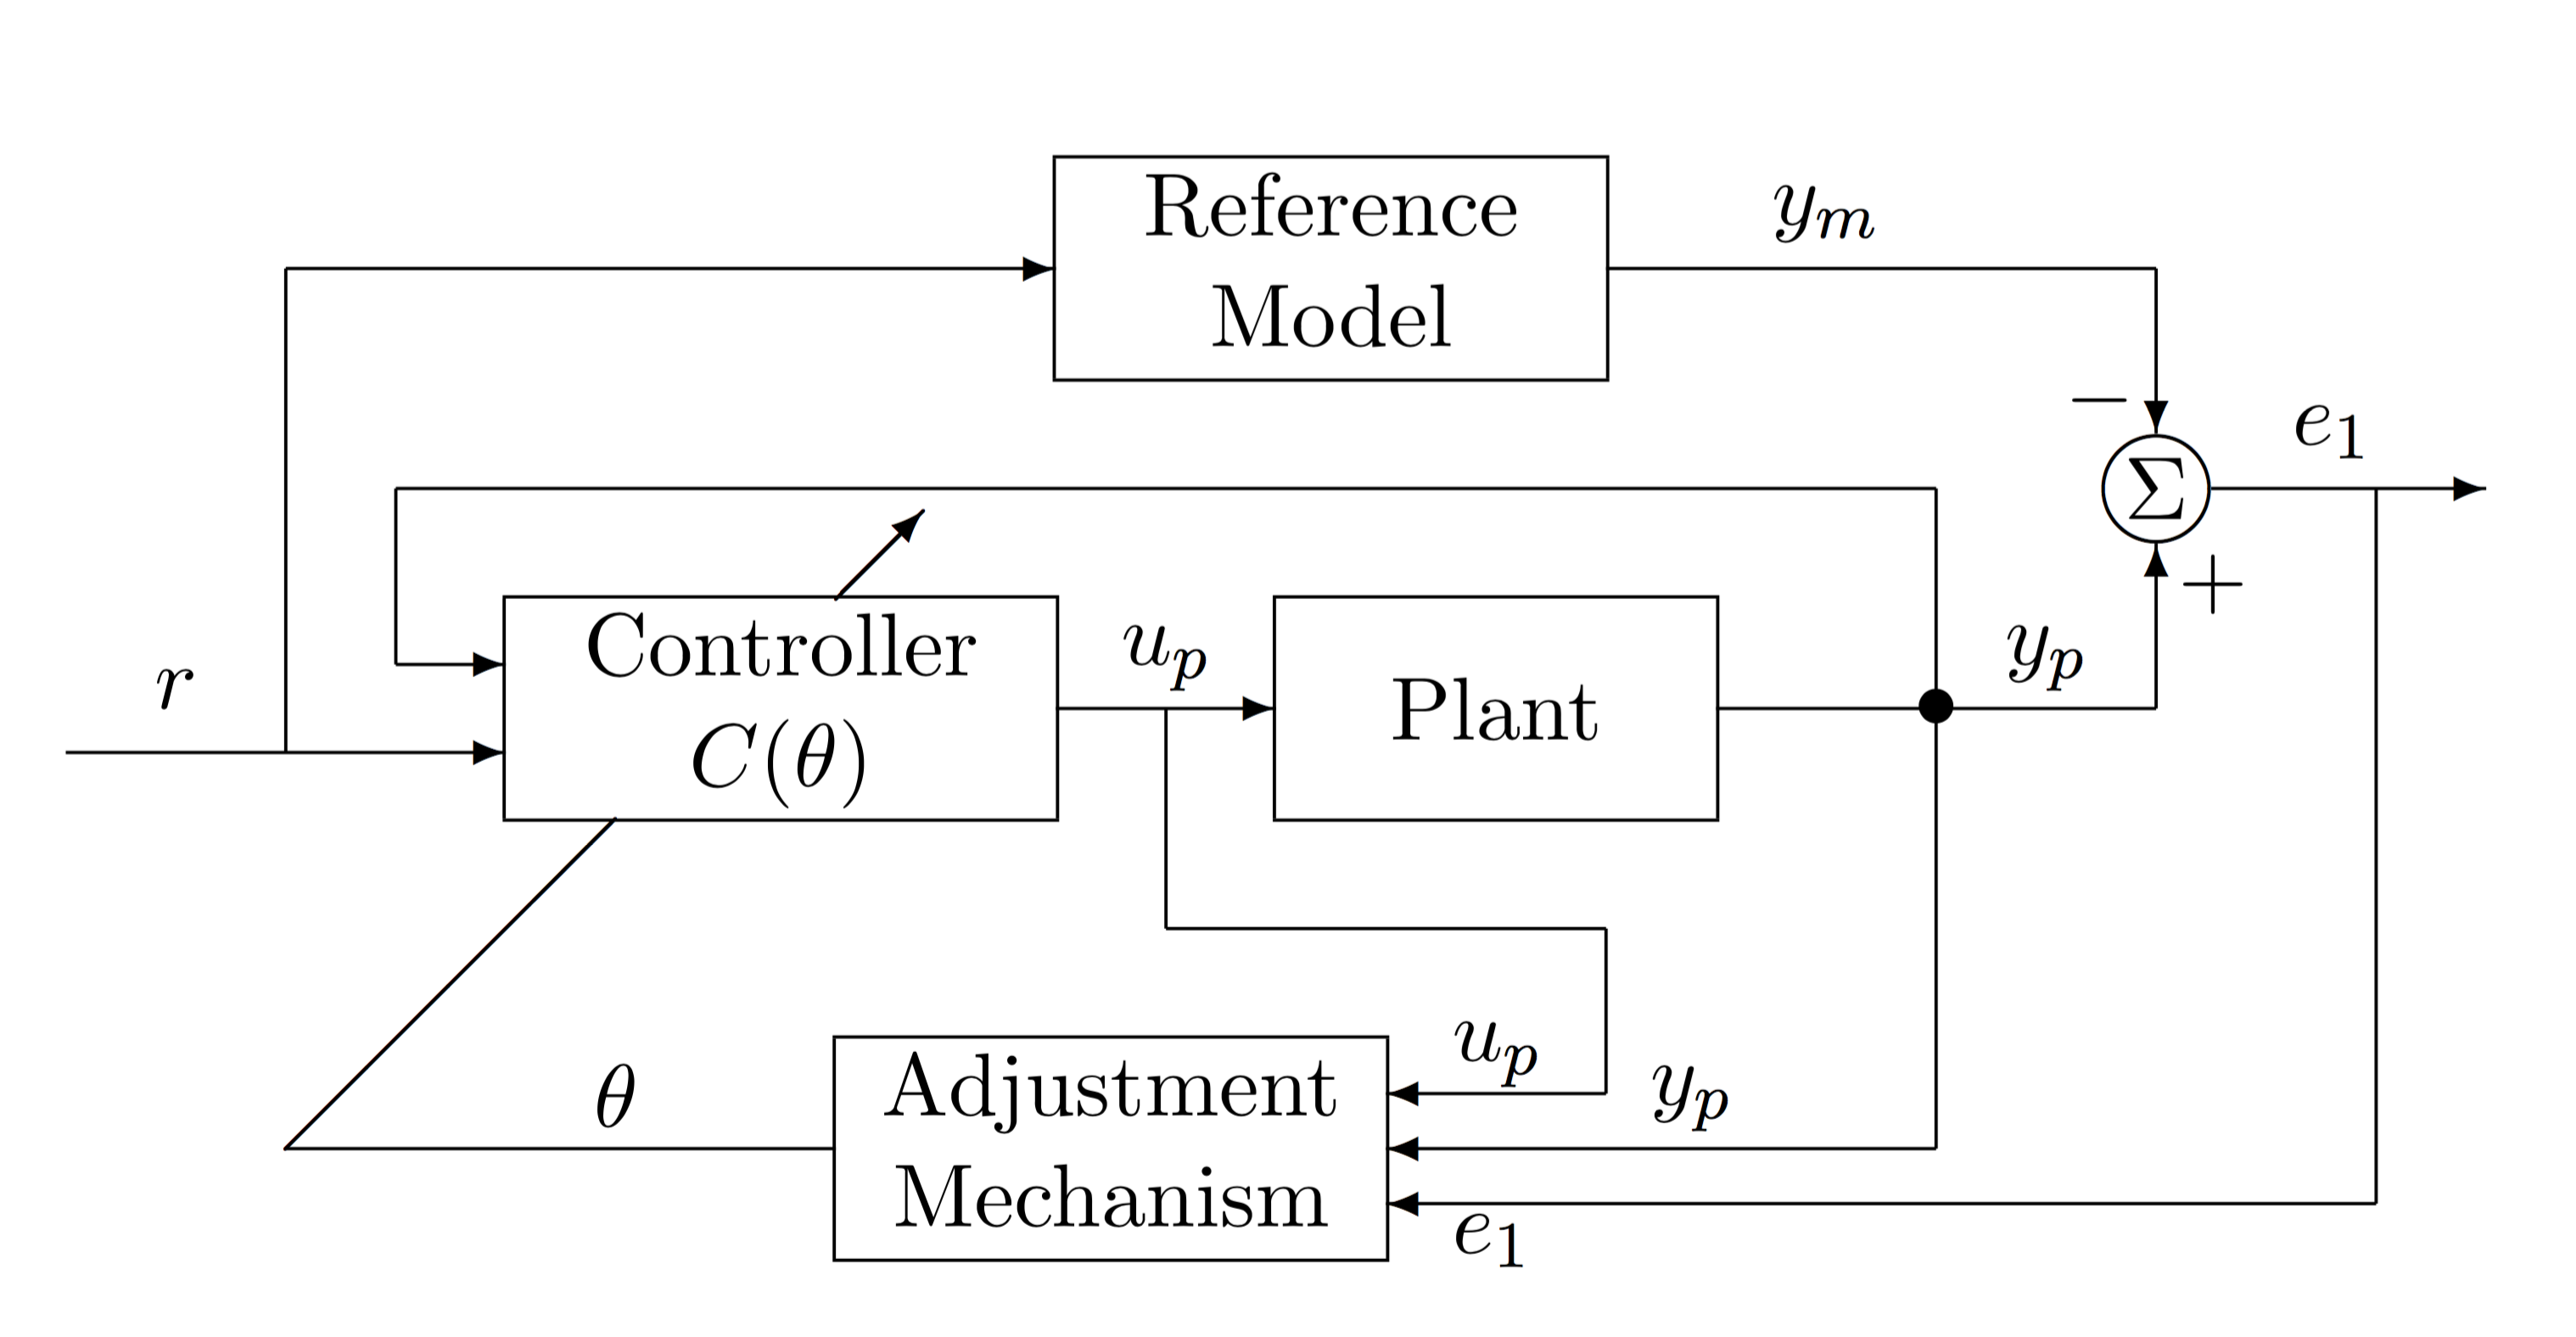
\includegraphics[width = \textwidth]{MRAC}
\caption{MRAC structure}
\label{fig:MRAC}
\end{center}
\end{figure}

\subsection{How to... MRAC}
Given a plant $y(s) = \frac{b}{s+a}u(s)$ and a reference model $y_m(s) = \frac{b_m}{s+a_m}r$ where $r \in L_\infty$.
Then the optimal ideal controller has the structure $u^* = -\theta_1^* y + \theta_2^* r$, where $\theta_1^*$ and $\theta_2^*$ is optimal controller parameters. The optimal parameters can be found by comparison between $y$ and $y_m$:
\begin{equation}
\begin{split}
y &= \frac{b}{s+a}(-\theta_1^* y + \theta_2^* r) \\
y(1+\frac{b\theta_1^*}{s+a} ) &= \frac{b\theta_2^*}{s+a}r \\
y &= \frac{b\theta_2^*}{s+a+b\theta_1^*}r
\end{split}
\end{equation}
which gives us $\theta_1^* = \frac{a_m-a}{b}$ and $\theta_2^* = \frac{b_m}{b}$. The closed loop differential equations is

\begin{equation}
\begin{split}
\dot{y} &= -ay +bu \\
& =-ay + b (-\theta_1 y + \theta_2 r) \\
& = (-a- b \theta_1) y + b \theta_2 r \\
\dot{y_m} &= -a_m y_m + b_m r
\end{split}
\end{equation}
We now define $e \triangleq y - y_m$, $\tilde{\theta_1}  \triangleq \theta_1 - \theta_1^*$, $\tilde{\theta_2}  \triangleq \theta_2 - \theta_2^*$ and derive the error dynamics.

\begin{equation}
\begin{split}
\dot{e} &= \dot{y}-\dot{y_m} \\
&= (-a- b \theta_1) y + b \theta_2 r - ( -a_m y_m + b_m r ) \\
&= -a_m y +  a_m y_m + (-a + a_m- b \theta_1) y + b \theta_2 r - b_m r \\
&= -a_m e + (-a + a_m- b (\tilde{\theta_1} +\frac{a_m-a}{b})) y + b (\tilde{\theta_2} + \frac{b_m}{b})r - b_m r \\
&= -a_m e - \tilde{\theta_1}b y + \tilde{\theta_2}b r
\end{split}
\end{equation}
We now use a Lyapunov (ish?) function $V = \frac{1}{2}e^2 + \frac{b}{2\gamma_1}\tilde{\theta_1^2} + \frac{b}{2\gamma_2}\tilde{\theta_2^2} $.

\begin{equation}
\begin{split}
\dot{V} &= e\dot{e} 	+ \frac{b}{\gamma_1}\tilde{\theta_1}\dot{\tilde{\theta_1}} 
				+ \frac{b}{\gamma_2} \tilde{\theta_2}\dot{\tilde{\theta_2}} \\
&= 	e (-a_m e - \tilde{\theta_1}b y + \tilde{\theta_2}b r) 
	+ \frac{b}{\gamma_1}\tilde{\theta_1}\dot{\theta_1} 
	+ \frac{b}{\gamma_2}\tilde{\theta_2}\dot{\theta_2} \\
&= -a_m e^2 	+ \frac{b}{\gamma_1}\tilde{\theta_1}(\dot{\theta_1}  - \gamma_1 y e)
			+ \frac{b}{\gamma_2}\tilde{\theta_2}(\dot{\theta_2} + \gamma_2 r e )
\end{split}
\end{equation}
The update laws are selected such that the derivative Lyapunov function are negative semi-definite.

\begin{equation}
\begin{split}
(\dot{\theta_1}  - \gamma_1 y e) &= 0 \Rightarrow \dot{\theta_1} = \gamma_1 y e \\
(\dot{\theta_2} + \gamma_2 r e ) &= 0 \Rightarrow \dot{\theta_2} = \gamma_2 r e
\end{split}
\end{equation}
It can now be shown that $e,\tilde{\theta_1}, \tilde{\theta_2},r,y_m,y,\dot{e} \in L_\infty$ and $e \in L_2$, which leads to $\lim_{t \to \infty} e(t) \rightarrow 0$ from Lemma 3.2.5.